\chapter{Design of the proposed solution}
\label{ch:DesignOfTheProposedSolution}
\lettrine[lraise=-0.1, lines=2, loversize=0.2]{L}{o}rem itsum
% El planificador desarrollado en esta tésis se compone a su vez de dos módulos bien diferenciados, el primero es el planificador de tareas propiamente dicho, encargado de la planificación de la misión y de su replanificación cuando fuera necesario, el segundo se encuentra a bordo de cada UAV y gestiona el comportamiento de cada equipo, ejecutando el plan que le ha asignado el primer módulo y reaccionando ante cualquier imprevisto de forma segura.

%%% Capi: En los capítulos 3 y 4 puedes coger texto del documento que tenemos hecho con Giuseppe, y del proyecto tuyo de tesis. 

% Se utilizará una aproximación jerárquica, con un planificador de alto nivel encargado de activar distintos controladores de bajo nivel. El planificador de alto nivel detectará las tareas requeridas por los operarios, y las distribuirá de manera centralizada entre los UAVs, planificando las recargas necesarias. Además, este planificador reaccionará en tiempo real ante posibles fallos reasignando tareas y ejecutando planes de contingencia. También tendrá capacidades cognitivas para interaccionar con humanos de manera eficiente. Los planificadores de bajo nivel se encargarán de controlar el movimiento de los UAVs para ejecutar las distintas tareas, por ejemplo volar hacia un lugar a inspeccionar o a la posición de un operario esperando una herramienta. La investigación de la tesis estará centrada en la planificación de alto nivel, y se utilizarán algoritmos del estado del arte para los controladores de bajo nivel.

% Del WP7_Scenarios: Modificar parámetros de una tarea
Once a task has been delivered to the High-Level Planner, in order to change any of its parameters, the Gesture Recognition node should send again the task, keeping the same Task ID and updating only the corresponding parameters. Thus, the High-Level Planner would overwrite it and allocate it again with the new parameters. In the following, a brief description on how to carry out each of the available tasks in the system. It is assumed that there are Low-Level Controllers running on the \glspl{ACW} to perform basic navigation actions, formation control for human worker monitoring, inspection operations, and physical interaction with the human worker (e.g., to pick or deliver a tool). These Low-Level Controllers operate in a known environment, represented by a map (i.e., an occupancy grid map) that also includes the position of obstacles and the power tower.


\section{Node diagram}
\label{sec:NodeDiagram}
%%% Explicar las comunicaciones que hay entre el planner y el manager
%%% Explicar que se ha hecho de forma que toda la inteligencia y las decisiones estén y se tomen en el planner

%% Informe de actividades: Node Diagram
% Desde la perspectiva del módulo implementado, la estructura de nodos se ve como está representado en la parte superior de la imagen. Se diferenciarían 3 conexiones distintas: la conexión con los módulos de nivel superior, la conexión con los controladores de bajo nivel, y la comunicación con los UAV. A su vez, el módulo marcado como n.2 se compone de dos partes, el planificador de tareas, que es un nodo centralizado, y que se encargará principalmente del reparto óptimo de tareas; y los nodos agente, de los cuales habrá una instancia por cada UAV y se ejecutarán sobre cada uno de ellos. La idea es que a través de la interfaz i.1, el n.2.1 reciba asíncronamente tareas provenientes de los módulos de mayor nivel, n.1. La información se propaga también de forma asíncrona hacia n.2.2 y los controladores de bajo nivel. Se consideran dos tareas posibles, “Monitor” e “Inspect”. Dependiendo de la tarea, a través de i.1, i.2 e i.3 viajarán unos datos u otros. Las flechas que conectan los nodos en el diagrama indican la direccionalidad de la comunicación, pudiendo haber comunicaciones unidireccionales o bidireccionales entre nodos.

%% Del WP7_Scenarios: diagrama de nodos y explicacion de los nodos y la informacion intercambiada
Figure \ref{fig:WP7scheme} shows the software architecture in WP7 from a task planning perspective, including the modules involved and their interfaces. High-level decision-making is carried out by two modules: the \textit{High-Level Planner} and the \textit{Agent Behavior Manager}. 

\begin{figure}[ht]
    \hspace{-1cm}
	\scalebox{0.7}{
		\begin{tikzpicture}
    		% WP7 block
    		\node (WP7-Box) at (8.35,0) [fill=gray!3,rounded corners, draw=black!70, densely dotted, minimum height=5cm, minimum width=19.5cm]{}; 
    		
    		% Gesture Recognition
    		\node (GestureRecognition) at (0,0) [text centered, fill=white, draw, rectangle, minimum width=1.5cm, text width=5.5em]{Gesture\\Recognition};
    		
    		\draw[-latex] ($(GestureRecognition) - (1.8,0)$) -- (GestureRecognition);
    		
    		% High-Level Planner
    		\node (HighLevelPlannerBox) at ($(GestureRecognition) + (3.5,0.25)$) [fill=yellow!15,rounded corners, draw=black!70, densely dotted, minimum height=2cm, minimum width=2.5cm]{}; 
    		\node (HighLevelPlanner) at ($(HighLevelPlannerBox) + (0,-0.25)$) [text centered, fill=white, draw, rectangle, minimum width=1.5cm, text width=5.5em]{High-Level\\Planner};
    		\node (Centralized) at ($(HighLevelPlanner) + (0,0.75)$) [text centered]{\small Centralized};
    		
    		\draw[-latex] (GestureRecognition.east) -- node[above]{Task} (HighLevelPlanner);
    		
    		%%%%%%%%%%%%%%%%%%%
    		% UAV 1
    		\node (UAV1) at ($(HighLevelPlanner) + (6.75,1.25)$) [fill=yellow!15,rounded corners, draw=black!70, densely dotted, minimum height=1.7cm, minimum width=5cm]{}; 
    		\node (AgentBehaviourManager1) at ($(UAV1) + (0,-0.25)$) [fill=white, draw, rectangle, text centered, text width=12em]{Agent Behaviour Manager};
    		\node (UAV1-Text) at ($(AgentBehaviourManager1) + (0,0.75)$) [text centered]{\small On board ACW-$1$};	

    		\draw[fill=black] ($ (HighLevelPlanner.east) + (1.715,0) $) arc(-180:180:0.05);
    		\draw[-latex] (HighLevelPlanner.east) -- ($ (HighLevelPlanner.east) + (1.75,0) $) -- ($ (HighLevelPlanner.east) + (1.75,1) $) -- node[above]{Task} node[below]{List} (AgentBehaviourManager1.west);
    		\draw[-latex] ($ (HighLevelPlanner.east) + (1.75,0) $) -- node[above]{Feedback} (HighLevelPlanner.east);
    		
    		%%%%%%%%%%%%%%%%%%%
    		
    		% Dots
    		\node (Dots2) at ($(UAV1) + (0,-1.25)$) [text centered]{\dots};
    		
    		%%%%%%%%%%%%%%%%%%%
    		
    		% UAV N
    		\node (UAVN) at ($(HighLevelPlanner) + (6.75,-1.25)$) [fill=yellow!15,rounded corners, draw=black!70, densely dotted, minimum height=1.7cm, minimum width=5cm]{}; 
    		\node (AgentBehaviourManagerN) at ($(UAVN) + (0,-0.25)$) [fill=white, draw, rectangle, text centered, text width=12em]{Agent Behaviour Manager};
    		\node (UAVN-Text) at ($(AgentBehaviourManagerN) + (0,0.75)$) [text centered]{\small On board ACW-$N$};	

    		\draw[-latex] (HighLevelPlanner.east) -- ($ (HighLevelPlanner.east) + (1.75,0) $) -- ($ (HighLevelPlanner.east) + (1.75,-1.5) $) -- node[above]{Task} node[below]{List} (AgentBehaviourManagerN.west);
    		
    		%%%%%%%%%%%%%%%%%%%
    		
    		% Lower-Level Controllers
    		\node (LowerLevelControllers) at ($(HighLevelPlanner) + (13.25,0)$) [text centered, fill=white, draw, rectangle, minimum width=1.5cm, text width=5.5em]{Lower-Level\\Controllers};
    		
    		\draw[-latex] (LowerLevelControllers.east) -- ($(LowerLevelControllers) + (1.8,0)$);
    		
    		\draw[fill=black] ($ (LowerLevelControllers.west) + (-1.535,0) $) arc(-180:180:0.05);
    		\draw[-latex] (AgentBehaviourManager1.east) -- ($ (LowerLevelControllers.west) + (-1.5,1) $) -- ($ (LowerLevelControllers.west) + (-1.5,0) $) --  node[above]{Task}
    	    node[below]{Params}	(LowerLevelControllers.west);
    		\draw[-latex] (LowerLevelControllers.west) -- ($ (LowerLevelControllers.west) + (-1.5,0) $) -- ($ (LowerLevelControllers.west) + (-1.5,1) $) -- node[above]{Task}
    	    node[below]{Result}	(AgentBehaviourManager1.east);
    		\draw[-latex] (AgentBehaviourManagerN.east) -- ($ (LowerLevelControllers.west) + (-1.5,-1.5) $) -- ($ (LowerLevelControllers.west) + (-1.5,0) $) -- (LowerLevelControllers.west);
    		\draw[-latex] (LowerLevelControllers.west) -- ($ (LowerLevelControllers.west) + (-1.5,0) $) -- ($ (LowerLevelControllers.west) + (-1.5,-1.5) $) -- 
    		node[above]{Task}
    		node[below]{Result} (AgentBehaviourManagerN.east);
    		
    		%%%%%%%%%%%%%%%%%%%%%
    		
    		\node (RealUAVs) at ($(WP7-Box.south) + (2,-1.25)$) [text centered, fill=white, draw, rectangle, minimum width=1.5cm, text width=6em]{ACWs\\autopilot};
    		\node (Humans) at ($(WP7-Box.south) + (-2,-1.25)$) [text centered, fill=white, draw, rectangle, minimum width=1.5cm, text width=6em]{Humans\\Tracker};
    		
    		\draw[-latex] (RealUAVs.north) -- node[right]{Pose, Battery, State} ($(WP7-Box.south) + (2,0)$);
    		\draw[-latex] ($(WP7-Box.south) + (2,0)$) -- (RealUAVs.north);
    		\draw[-latex] (Humans.north) -- node[left]{Pose} ($(WP7-Box.south) + (-2,0)$);
		
	    \end{tikzpicture}}
	\caption{WP7 Software architecture: Modules and interfaces.}
	\label{fig:WP7scheme}
\end{figure}

The \textit{High-level Planner} is the centralized module of the software architecture and runs on a ground station. This module is in charge of task planning, i.e., it decides which tasks will be assigned to each \gls{ACW}. The system knows the available \glspl{ACW} thanks to the feedback provided by the Terabee~ \gls{RTPS}. At this stage, battery constraints and \gls{ACW} positions and capabilities are taken into consideration. Such information is supplied at a constant rate (to be defined). The number and type of available \glspl{ACW} can be specified before the mission starts via a configuration file. 

The \textit{Agent Behavior Manager} is a distributed module running on board each \gls{ACW}. This module mainly runs a state machine implemented as a \gls{BT} which governs the \gls{ACW} to perform each of the assigned tasks. Each \gls{BT} monitors the \gls{ACW}'s battery and task status and reacts to any possible failure or unexpected event, requesting a new re-planning to the High-Level Planner in case of need. In addition, the \textit{ACW autopilot} and \textit{Human Tracker} nodes supply for the ACW state and human worker pose, respectively. This information is used for monitoring and tool delivery tasks.  

The data interfaces for each module in the software architecture are listed in Table~\ref{tab:interfaces}, while the data explanation is provided in Table~\ref{tab:shareddata}.

\begin{table}[ht]
    \centering
    \caption{Description of the data interfaces for each software module.}
    \label{tab:interfaces}
    \small
    \begin{tabular}{|p{0.25\columnwidth}|p{0.25\columnwidth}|p{0.4\columnwidth}|}
      \hline
      \multicolumn{1}{|c}{\textbf{Module Name}} & \multicolumn{1}{|c|}{\textbf{Input Data}} & \multicolumn{1}{c|}{\textbf{Output Data}}\\ \hline \hline
      Gesture Recognition & Images & \textbf{Task, defined by:} Task ID, Task Type, Monitoring Distance, Monitoring Number, WP List, Tool ID (some task parameters will be ignored depending on Task Type) \\ \hline
      
      High-Level Planner & Task, Feedback (Agent Beacon, BatteryEnough, \gls{BT} info), Humans' Pose, \glspl{ACW}' Pose, Battery and State & Task List adding to each one its extra parameters result of the planning (Formation and/or List of \glspl{ACW}' IDs) \\\hline
      
      Agent Behaviour Manager & Task List, Result (Low-Level Result), Human Pose, \glspl{ACW} Pose, Battery and State & Params needed by Low-Level Controllers (depending on Task Type) \\ \hline
      
      Low-Level Controllers & Params (depending on Task Type) & Result \\ \hline
      
      Humans Tracker &  & Pose \\ \hline
      
      \gls{ACW} autopilot & Low-Level orders & Pose, Battery and State \\ \hline
      
    \end{tabular}
\end{table}
  
\begin{table}[htb]
    \centering
    \caption{Description of data types.}
    \label{tab:shareddata}
    \small
    \begin{tabular}{|p{0.2\columnwidth}|p{0.15\columnwidth}|p{0.55\columnwidth}|}
      \hline
      \multicolumn{1}{|c}{\textbf{Data name}} & \multicolumn{1}{|c|}{\textbf{Data type}} & \multicolumn{1}{c|}{\textbf{Comment}} \\ \hline \hline
      
      Task ID & String & Unique identifier of each task \\ \hline
      
      Task Type & Integer & Task type indicator: m/M, i/I or d/D \\ \hline
      
      Human Target ID & String & Unique identifier of each human worker. The position of the human target and other needed info is supposed to be known and accessible via its ID. \\ \hline
      
      Monitoring Distance & Float & Distance from which the \gls{ACW} surveil the worker during a safety monitoring task \\ \hline
      
      Monitoring Number & Integer & Number of \glspl{ACW} that are required in formation for a certain safety monitoring task \\ \hline
      
      WP List & List of $3$ float tuples ($x$, $y$, and $z$) & List of waypoints to be inspected \\ \hline
      
      List of \glspl{ACW}' IDs & List of Strings & List of the unique identifiers of the \glspl{ACW} that have been selected for a task that requires multiple \glspl{ACW} \\ \hline
      
      Formation & Integer & Indicates which of the predefined types of formations should be used for monitoring (e.g., circle, triangle) \\ \hline
      
      Tool ID & String & Unique identifier of the tool to be delivered \\ \hline
      
      \gls{ACW} Pose & geometry\_msgs /PoseStamped & \gls{ACW} Position and orientation \\ \hline
      
      \gls{ACW} Battery & sensors\_msgs /BatteryState & Percentage of battery in the \gls{ACW}\\ \hline
      
      Battery Enough & Boolean & Result of computing if an \gls{ACW} will have enough battery for its current task \\ \hline
      
      Agent Beacon & String, Integer & \gls{ACW} unique ID and integer defining the type of \gls{ACW} (Safety, Inspect, or Physical Interaction). Used as heartbeat to detect new \glspl{ACW} \\ \hline
      
      \gls{BT} info & String list & Status of each \gls{BT} node: which are Running, which are IDLE, which just returned SUCCESS, and which just returned FAILURE \\ \hline
      
      Lower-Level Result & Boolean & Result of the Low-Level Controllers after a call \\ \hline
      
    \end{tabular}
\end{table}

\section{Centralized module: task planner}
\label{sec:Centralized module:TaskPlanner}
%% Protocolo de desconexión
%% Protocolo de pérdida de batería
%% Que ocurre cuando una tarea termina
%% Replanificaciones de tareas: restricciones a la hora de planificar o replanificar

%% Informe de actividades: Task Planner
% Este nodo está pensado para que se ejecute de forma centralizada y se comunique con cada uno de los UAVs disponibles. Se encarga principalmente de organizar el reparto de tareas, pero también tiene otras labores secundarias como son realizar la escucha y seguimiento de las balizas que envían los UAVs a modo de latidos o “heartbeat”, subscribirse a la información necesaria de los sensores de cada uno de los UAVs, comprobar si la batería de cada UAV es suficiente para completar el plancompleto de tareas asignado y atender a la información que le envía el nodo “Agent” con información sobre el estado del BT.

\section{Distributed module: behavior manager}
\label{sec:Distributed module: behavior manager}
%%% Explicar que se ha hecho con árboles de comportamiento en paralelo a algunos procesos de ros

%% Informe de actividades: Máquinas de estados vs árboles de comportamiento
% Una vez asimilado el contexto y los requisitos del proyecto, y antes de proceder con el diseño de la solución, se dedicó un tiempo a estudiar las diferencias entre las máquinas de estados finitas (FSM), con las cuales se estaba familiarizado en aquel momento, y los árboles de comportamiento (BT), de los cuales se desconocía completamente su existencia y funcionamiento. Durante este tiempo no solo se prestó atención a las ventajas e inconvenientes de cada herramienta, sino que también se estudiaron las diferentes librerías para C++, preferiblemente compatibles con ROS, que estaban disponibles [1][2][3][4] y se valoró la calidad de la documentación, la cantidad de ejemplos, cruciales para aprender rápidamente a usar una librería cuando aún se es un usuario poco experimentado del lenguaje de programación, la facilidad de uso y el soporte de la librería entre otras cosas. Aunque la cantidad de personas que emplean librerías de FSM es mayor que en el caso de los BT, y por tanto, es mucho más probable encontrar información en foros de Internet relativa a algún detalle concreto que se necesite y que no esté bien documentado, las ventajas que ofrecen los árboles de comportamiento frente a las máquinas de estado finitas fueron determinantes para decidir emplear este tipo de arquitecturas. Tras una primera formación empleando una librería para BT que ya había sido usada puntualmente por un miembro del grupo [2], se descartó como librería a emplear por la escasa documentación y la falta de características que se consideraban necesarias. Finalmente se encontró una librería que parecía tener una documentación bastante mejor, soporte y mantenimiento aún activos y ejemplos simples de código que se podían emplear como punto de partida [3], y que además venía acompañada de una herramienta para diseñar BT gráficamente [4]. El punto negativoes que no parece tener aún muchos usuarios ni un apartado de preguntas y comentarios, y por tanto, ante cualquier problema o duda con la librería, no se dispondrá de ningún tipo de ayuda.

% Informe de actividades: Nodo Agent
% El nodo “Agent” se ejecuta sobre cada UAV, siendo su función principal la de ejecutar el árbol de comportamiento. En el código que implementa este nodo se encuentran definidos todos los nodos del BT, el código interno de cada uno de ellos. Además, este nodo se encarga de subscribirse a la información necesaria de los UAV, de mandar las balizas para comunicar al nodo “Planner” que se ha conectado, o que sigue conectado, de recibir balizas a su vez de este nodo para saber de esta forma cuándo él mismo se ha desconectado, de recibir la lista de tareas que asigna el nodo “Planner” al UAV sobre el cual se está ejecutando este nodo, y de llamar a los controladores de bajo nivel.

%% Informe de actividades: Diseño del árbol de comportamiento
% Diseñar el árbol de comportamiento no fue una labor trivial, ya que se estaba habituado a diseñar pensando en máquinas de estado, pero no pensando en árboles de comportamiento. Además, para cada comportamiento deseado no hay una única implementación posible, lo que hace más complicado el diseño cuando no se tiene la intuición suficiente para saber qué forma es mejor. Para tratar de ganar experiencia con la que desarrollar cierta intuición y los conocimientos necesarios para elaborar desde cero un BT, se dedicó un tiempo a reunir y estudiar toda la información posible sobre los árboles de comportamiento que se encontrara por Internet [5][6][7]. Esto fue posible gracias a que los BT sí que son algo más común en el desarrollo de videojuegos [7]. El diseño del BT no ha permanecido invariante desde que se hizo, sino que ha sufrido modificaciones puntuales fruto de reuniones y revisiones del trabajo. Estas modificaciones principalmente buscaban solucionar algún problema detectado ya fuera en algún re-estudio teórico o tras la observación de algún comportamiento indeseado en pruebas de simulación. Antes mostrar y proceder con la explicación del funcionamiento del diseño de BT propuesto, se comentarán brevemente los tipos de nodos disponibles en la librería seleccionada y el funcionamiento de cada uno de ellos.

%% Informe de actividades: Tipos de nodos de BT
\begin{figure}[htbp]
    \centering
    \subfloat[]{%Fallback
		\label{subfig:Fallback}
        
\begin{tikzpicture}
			\node (MainTree) at (0,0) [text centered, fill=white, draw, rectangle, minimum width=0.5cm, text width=0.5em]{\textbf{?}};
		\end{tikzpicture}}
    \hfill
    \subfloat[]{%Sequence
		\label{subfig:Sequence}
        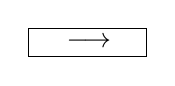
\begin{tikzpicture}
			\node (MainTree) at (0,0) [text centered, fill=white, draw, rectangle, minimum width=1.5cm, text width=1.5em]{$\longrightarrow$};
		\end{tikzpicture}}
	\hfill
    \subfloat[]{%Reactive
		\label{subfig:Reactive}
        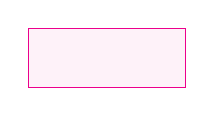
\begin{tikzpicture}
			\node (MainTree) at (0,0) [text centered, fill=magenta!5, draw=magenta, rectangle, minimum width=2cm, minimum height=0.75cm, text width=2em]{};
		\end{tikzpicture}}
    \hfill
    \subfloat[]{%Common
		\label{subfig:Common}
        \begin{tikzpicture}
			\node (MainTree) at (0,0) [text centered, fill=white, draw, rectangle, minimum width=2cm, minimum height=0.75cm, text width=2em]{};
		\end{tikzpicture}}
    \hfill
    \subfloat[]{%Decorator
		\label{subfig:Decorator}
        
\begin{tikzpicture}
			\node (MainTree) at (0,0) [text centered, fill=orange!5, draw=orange, rectangle, minimum width=2cm, minimum height=0.75cm, text width=2em]{};
		\end{tikzpicture}}
    \hfill
    \subfloat[]{%Action
		\label{subfig:Action}
		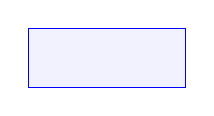
\begin{tikzpicture}
			\node (MainTree) at (0,0) [text centered, fill=blue!5, draw=blue, rectangle, minimum width=2cm, minimum height=0.75cm, text width=2em]{};
		\end{tikzpicture}}
		\hfill
    \subfloat[]{%Condition
		\label{subfig:Condition}
        \begin{tikzpicture}
			\node (MainTree) at (0,0) [text centered, fill=blue!5, draw=blue, ellipse, minimum width=2cm, minimum height=0.75cm, text width=2em]{};
		\end{tikzpicture}}
    \caption{Different types of nodes that can be present in an \gls{BT}}
    \label{fig:CounterRunImagenes}
\end{figure}
% El nodo tipo \ref{subfig:Fallback} es un nodo de control de decisión, en inglés llamado “Fallback”. Su comportamiento es el de llamar uno a uno a cada uno de sus hijos, de izquierda a derecha, hasta que uno devuelve “SUCCESS”, devolviendo él también “SUCCESS”, o devolviendo “FAILURE” en caso de que todos sus hijos devuelvan “FAILURE”. El nodo \ref{subfig:Sequence} es un node de control del tipo secuencia. Cuando un hijo devuelve “SUCCESS”, llama al siguiente. En caso de que algunodevuelva “FAILURE”, la secuencia se para y el nodo devuelve también “FAILURE”. Si todos lo hijos se han ejecutado y han devuelto “SUCCESS”, el nodo también devuelve “SUCCESS”. Si el nodo es del color de \ref{subfig:Reactive}, significa que es un nodo reactivo, lo que significa que, aunque un hijo esté ejecutándose, se re-evalúan los hijos previos. El color \ref{subfig:Common} es para los nodos normales. Si un hijo devuelve “RUNNING”, se le vuelve a llamar en la ejecución siguiente. En azul se representan los nodos sin hijos, que pueden ser del tipo \ref{subfig:Condition}, que es un nodo para comprobar una condición, o del tipo \ref{subfig:Action}, que ejecuta una acción. Por último, en color \ref{subfig:Decorator} se representan los nodos decoradores, cuyo comportamiento dentro del BT es programable.

%% Del WP7_Scenarios
Behaviour Trees are a more advanced mechanism to implement Finite State Machines, working like them but with improvements in terms of composability, configurability and reusability. Behaviour Trees are made up of control nodes, decorator nodes, and leaf nodes. Control nodes could be either \textit{Fallback} nodes (represented with a question mark), which try success calling one by one each of their children, or \textit{Sequence} nodes (represented with an arrow), which call their children in order if the previous one have returned success. Fallback nodes return success if one of its children does it, failure if none of them return success, and running if a children returns running. On the other hand, Sequence nodes return success when all children have been called in order and have returned success. If any of them returns failure, the sequence is broken and the sequence node returns failure too. When a child returns running, sequence node does it too. A control node could also be \textit{Reactive} (represented in a purple box), which means that its already called children are called again in the next iteration. A child node could be another control node, a decorator node or a leaf node. A decorator node (represented in an orange box) can only have one child (of any type) and its function is programmable (e.g., modifying its child result or retrying calling its child a number of times). Leaf nodes could be condition nodes (represented in an elliptical shaped box) that check a condition and return either success or failure, or action nodes (represented in a rectangular box) that take longer to execute and could also return running).


\subsection{Main tree}
\label{sec:MainTree}
%%% Recalcar que se ha hecho de forma que toda la inteligencia y las decisiones estén y se tomen en el planner
%%% Hablar aqui dentro de como se gestionan las desconexiones, la batería y las replanificaciones
%% Protocolo de desconexión
%% Protocolo de pérdida de batería
%% Que ocurre cuando una tarea termina

%% Del WP7_Scenarios: main tree
\begin{figure}[ht]
	\begin{center}
		\scalebox{0.9}{
			\begin{tikzpicture}
        		\node (MainTree) at (0,0) [text centered, fill=white, draw, rectangle, minimum width=1.5cm, text width=5.5em]{Main Tree};

        		\node (RootFallback) at ($(MainTree) + (0,-1)$) [text centered, fill=magenta!5, draw=magenta, rectangle, minimum width=0.5cm, text width=0.5em]{\textbf{?}};
        		\draw[-latex] (MainTree.south) -- (RootFallback.north);

        		\node (MissionOverSequence) at ($(RootFallback) + (-3,-1.5)$) [text centered, fill=white, draw, rectangle, minimum width=1.5cm, text width=1.5em]{$\longrightarrow$};
        		\draw[-latex] (RootFallback.south) -- (MissionOverSequence.north);
        		\node (ForceRunning) at ($(RootFallback) + (3, -1.5)$) [text centered, fill=orange!5, draw=orange, rectangle, minimum width=1.5cm, text width=5.5em]{Force Running};
        		\draw[-latex] (RootFallback.south) -- (ForceRunning.north);
        		
        		\node (MissionOver) at ($(MissionOverSequence) + (-1.75,-1.5)$) [text centered, fill=blue!5, draw=blue, ellipse, minimum width=1.5cm, text width=5.5em]{Mission Over?};
        		\draw[-latex] (MissionOverSequence.south) -- (MissionOver.north);
        		\node (BackToStation) at ($(MissionOverSequence) + (1.75, -1.5)$) [text centered, fill=blue!5, draw=blue, rectangle, minimum width=1.5cm, text width=5.5em]{Back To Station};
        		\draw[-latex] (MissionOverSequence.south) -- (BackToStation.north);
        		\node (MissionFallback) at ($(ForceRunning) + (0,-1.5)$) [text centered, fill=magenta!5, draw=magenta, rectangle, minimum width=0.5cm, text width=0.5em]{\textbf{?}};
        		\draw[-latex] (ForceRunning.south) -- (MissionFallback.north);

        		\node (IdleSequence) at ($(MissionFallback) + (-4.25,-1.25)$) [text centered, fill=magenta!5, draw=magenta, rectangle, minimum width=1.5cm, text width=1.5em]{$\longrightarrow$};
        		\draw[-latex] (MissionFallback.south) -- (IdleSequence.north);
        		\node (WaitFallback) at ($(MissionFallback) + (4.25,-1.25)$) [text centered, fill=magenta!5, draw=magenta, rectangle, minimum width=0.5cm, text width=0.5em]{\textbf{?}};
        		\draw[-latex] (MissionFallback.south) -- (WaitFallback.north);
        		
        		\node (Inverter) at ($(IdleSequence) + (-3, -1.5)$) [text centered, fill=orange!5, draw=orange, rectangle, minimum width=1.5cm, text width=5.5em]{Inverter};
        		\draw[-latex] (IdleSequence.south) -- (Inverter.north);
        		\node (TaskSequence) at ($(IdleSequence) + (2.5,-1.5)$) [text centered, fill=magenta!5, draw=magenta, rectangle, minimum width=1.5cm, text width=1.5em]{$\longrightarrow$};
        		\draw[-latex] (IdleSequence.south) -- (TaskSequence.north);
        		\node (IsBatteryFull) at ($(WaitFallback) + (-1.75,-1.5)$) [text centered, fill=blue!5, draw=blue, ellipse, minimum width=1.5cm, text width=5.5em]{Is Battery Full?};
        		\draw[-latex] (WaitFallback.south) -- (IsBatteryFull.north);
        		\node (Recharge) at ($(WaitFallback) + (1.75, -1.5)$) [text centered, fill=blue!5, draw=blue, rectangle, minimum width=1.5cm, text width=6.5em]{Recharge};
        		\draw[-latex] (WaitFallback.south) -- (Recharge.north);

        		\node (Idle) at ($(Inverter) + (0,-1.5)$) [text centered, fill=blue!5, draw=blue, ellipse, minimum width=1.5cm, minimum height=1.35cm, text width=5.5em]{Idle?};
        		\draw[-latex] (Inverter.south) -- (Idle.north);
        		\node (IsBatteryEnough) at ($(TaskSequence) + (-1.75,-1.5)$) [text centered, fill=blue!5, draw=blue, ellipse, minimum width=1.5cm, text width=5.5em]{Is Battery Enough?};
        		\draw[-latex] (TaskSequence.south) -- (IsBatteryEnough.north);
        		\node (PerformTaskTree) at ($(TaskSequence) + (1.75, -1.5)$) [text centered, fill=white, draw, rectangle, minimum width=1.5cm, text width=6.5em]{Perform Task Tree};
        		\draw[-latex] (TaskSequence.south) -- (PerformTaskTree.north);
        		
        		%\draw[-latex] (.south) -- (.north);
		    \end{tikzpicture}}
		\caption{Behavior Tree: Main tree}
		\label{fig:MainTree}
	\end{center}
	\vspace{-1em}
\end{figure}
%% Informe de actividades: Main tree
% Esta es la base del árbol de comportamiento implementado. Primeramente se comprueba que la misión no haya terminado, de forma que el BT siga ejecutándose hasta que esta finalice. En caso contrario se ejecuta el resto del árbol. En caso de que el UAV sobre el cual se ejecuta el BT tenga asignada alguna tarea, se comprueba si se tiene batería suficiente y en caso afirmativo se ejecuta el sub-árbol para las tareas. Si el UAV no tiene ninguna tarea asignada, se comprueba el nivel de batería y se recarga. Esta estructura está diseñada de forma que, si el UAV se desconecta, o si el nodo “isBatteryEnough” devuelve “FAILURE”, se vacía la cola de tareas asignada como plan al UAV en cuestión y este, al detectar en la siguiente iteración que se encuentra ocioso, “Idle”, se dirigirá de forma segura a recargar. En ambos casos, será ejecutada una re-planificación de tareas.

%% Del WP7_Scenarios: main tree
Each Agent Behavior Manager implements several interconnected \gls{BT}. The \emph{Main tree} is depicted in Fig.~\ref{fig:MainTree}. This \gls{BT} checks whether the mission is over (a mission would represent the working session, not a single task, i.e., whether the \gls{ACW} is ready to be turned off) and otherwise, whether the \gls{ACW} has any task to perform. If so, the battery level is checked and, depending on the result, either the corresponding task is executed (sub-tree represented in Fig.~\ref{fig:PerformTasksTree}) or the \gls{ACW} is guided to a recharging station\footnote{Both Safety, Inspection and Physical-ACW provide an input interface to guide the \gls{ACW} to the charging station. In other words, among the low-level controller capabilities, there is a "reach this point". The location of the charging stations is known in advance or provided as input by the High-Level Planner/Behavior Tree.}. The \gls{BT} is also prepared to be safe against a loss of connection with the centralized module. Both unexpected events are managed flushing the task queue for the \gls{ACW} to recharging, while giving the High-Level Planner control to decide when it is the best time to stop recharging (the High-Level Planner just needs to assign tasks again so that the \gls{ACW} start working back).

%% Del WP7_Scenarios: perform task tree
\begin{figure}[ht]
	\begin{center}
		\scalebox{0.75}{
			\begin{tikzpicture}
			    \node (PerformTaskTree) at (0,0) [text centered, fill=white, draw, rectangle, minimum width=1.5cm, text width=5.5em]{Perform Task Tree};
        		
        		\node (TaskFallback) at ($(PerformTaskTree) + (0,-1.5)$) [text centered, fill=magenta!5, draw=magenta, rectangle, minimum width=0.5cm, text width=1.5em]{\textbf{?}};
        		\draw[-latex] (PerformTaskTree.south) -- (TaskFallback.north);
        		
        		\node (MonitorSequence) at ($(TaskFallback) + (-7,-1.5)$) [text centered, fill=magenta!5, draw=magenta, rectangle, minimum width=1.5cm, text width=1.5em]{$\longrightarrow$};
        		\draw[-latex] (TaskFallback.south) -- (MonitorSequence.north);
        		\node (InspectSequence) at ($(TaskFallback) + (0,-1.5)$) [text centered, fill=magenta!5, draw=magenta, rectangle, minimum width=1.5cm, text width=1.5em]{$\longrightarrow$};
        		\draw[-latex] (TaskFallback.south) -- (InspectSequence.north);
        		\node (DeliverSequence) at ($(TaskFallback) + (7,-1.5)$) [text centered, fill=magenta!5, draw=magenta, rectangle, minimum width=1.5cm, text width=1.5em]{$\longrightarrow$};
        		\draw[-latex] (TaskFallback.south) -- (DeliverSequence.north);
        		
        		\node (IsTaskMonitor) at ($(MonitorSequence) + (-1.75,-2)$) [text centered, fill=blue!5, draw=blue, ellipse, minimum width=1.5cm, text width=6em]{Is Task "Monitoring"?};
        		\draw[-latex] (MonitorSequence.south) -- (IsTaskMonitor.north);
        		\node (MonitorTree) at ($(MonitorSequence) + (1.75, -2)$) [text centered, fill=white, draw, rectangle, minimum width=1.5cm, text width=6.5em]{Monitoring Task Tree};
        		\draw[-latex] (MonitorSequence.south) -- (MonitorTree.north);
        		\node (IsTaskInspect) at ($(InspectSequence) + (-1.75,-2)$) [text centered, fill=blue!5, draw=blue, ellipse, minimum width=1.5cm, text width=5.5em]{Is Task "Inspection"?};
        		\draw[-latex] (InspectSequence.south) -- (IsTaskInspect.north);
        		\node (InspectTree) at ($(InspectSequence) + (1.75, -2)$) [text centered, fill=white, draw, rectangle, minimum width=1.5cm, text width=5.5em]{Inspection Task Tree};
        		\draw[-latex] (InspectSequence.south) -- (InspectTree.north);
        		\node (IsTaskDeliver) at ($(DeliverSequence) + (-1.75,-2)$) [text centered, fill=blue!5, draw=blue, ellipse, minimum width=1.5cm, text width=5.5em]{Is Task "Tool Delivery"?};
        		\draw[-latex] (DeliverSequence.south) -- (IsTaskDeliver.north);
        		\node (DeliverTree) at ($(DeliverSequence) + (1.5, -2)$) [text centered, fill=white, draw, rectangle, minimum width=1.5cm, text width=6.5em]{Tool Delivery Task Tree};
        		\draw[-latex] (DeliverSequence.south) -- (DeliverTree.north);
        		
		    \end{tikzpicture}}
		\caption{Behavior Tree: Perform Task Tree}
		\label{fig:PerformTasksTree}
	\end{center}
\end{figure}
%% Informe de actividades: perform task tree
% Este es el sub-árbol para comprobar qué tarea es la que se debe ejecutar y llamar consecuentemente a uno u otro sub-árbol. En este punto se podrían llamar directamente a los módulos del nivel inferior, pero se decidió que el control no se le pasaría a los módulos de niveles inferiores hasta que el UAV se encuentre cerca de la zona donde haya de realizar su tarea.

%% Del WP7_Scenarios: subtrees
Figures \ref{fig:MonitorTree}, \ref{fig:InspectTree} and \ref{fig:DeliverToolTree} represent the sub-trees that run Safety, Inspection, and Physical tasks, respectively. They all guide the \gls{ACW} close to where the tasks needs to be performed (e.g., close to a worker to monitor or a place to inspect) and then, the corresponding Lower-Level Controller is called. These Lower-Level Controllers run on board the corresponding \gls{ACW}s and must communicate their results (success or failure) asynchronously back to the Agent Behavior Manager, so that the Behaviour Tree could continue running.

%% Informe de actividades: seguridad, emergencias y concentración de la inteligencia
% Destacar que este árbol de comportamiento no se encarga de realizar el reparto y la planificación de tareas a largo plazo como tal, sino que este se ejecuta sobre cada UAV y se encarga de llevar a cabo la ejecución del plan que se le ha asignado. Este BT es además el responsable de detectar, comunicar y actuar ante cualquier situación inesperada como un pronto agotamiento de la batería o una desconexión. A su vez, este submódulo se encarga de comunicar al planificador todos los detalles y los eventos que vayan sucediendo para que este decida si es necesario re-planificar toda la misión o no. El objetivo de este BT es conseguir que en los UAVs no haya toma de decisiones como tal, sino que toda la inteligencia se encuentre centralizada y que todos los comportamientos y decisiones que un UAV pueda llegar a tomar estén contenidas y precalculadas dentro de la estructura del propio BT, que está diseñado de forma que asegure el buen funcionamiento y la seguridad del equipo ante cualquier circunstancia.

% Information exchanges 
% Information interfaces/channels
% Takeovers
\subsection{Inspection task tree}
\label{sec:InspectionTaskTree}
% Del WP7_Scenarios
\textbf{High-Level Planner inputs}: Task ID, Task Type and Waypoint List (the rest will be ignored).

\textbf{Description}: the High-Level Planner, from the list of waypoints, will decide how many \glspl{ACW} are required and which part of the waypoint list is assigned to each one. Then, it would send to each corresponding Agent Behavior Manager the task parameters, including a list with the IDs of the selected~ glspl{ACW}. The same information is forwarded to the Lower-Level Controllers when the BT calls them (see Fig.~\ref{fig:InspectTree}). Basically, the list of waypoints to be inspected are covered by the assigned \glspl{ACW}, stopping at each of them to take images.  

\begin{figure}[ht]
	\begin{center}
		\scalebox{1}{
			\begin{tikzpicture}
			    \node (InspectTree) at (0,0) [text centered, fill=white, draw, rectangle, minimum width=1.5cm, text width=5.5em]{Inspection Task Tree};
        		
        		\node (InspectTaskSequence) at ($(InspectTree) + (0,-1.5)$) [text centered, fill=magenta!5, draw=magenta, rectangle, minimum width=1.5cm, text width=1.5em]{$\longrightarrow$};
        		\draw[-latex] (InspectTree.south) -- (InspectTaskSequence.north);
        		
        		\node (NearWPFallback) at ($(InspectTaskSequence) + (-1.5,-1.5)$) [text centered, fill=magenta!5, draw=magenta, rectangle, minimum width=0.5cm, text width=0.5em]{\textbf{?}};
        		\draw[-latex] (InspectTaskSequence.south) -- (NearWPFallback.north);
        		\node (Inspect) at ($(InspectTaskSequence) + (1.5,-1.5)$) [text centered, fill=blue!5, draw=blue, rectangle, minimum width=1.5cm, text width=5.5em]{Inspect};
        		\draw[-latex] (InspectTaskSequence.south) -- (Inspect.north);
        		
        		\node (IsUAVnearWP) at ($(NearWPFallback) + (-1.75,-2)$) [text centered, fill=blue!5, draw=blue, ellipse, minimum width=1.5cm, text width=5.5em]{Is \gls{ACW} near WP?};
        		\draw[-latex] (NearWPFallback.south) -- (IsUAVnearWP.north);
        		\node (GoNearWP) at ($(NearWPFallback) + (1.75, -2)$) [text centered, fill=blue!5, draw=blue, rectangle, minimum width=1.5cm, text width=6.5em]{Go near WP};
        		\draw[-latex] (NearWPFallback.south) -- (GoNearWP.north);
		    \end{tikzpicture}
		}
		\caption{Behavior Tree: sub-tree that controls the inspect tasks}
		\label{fig:InspectTree}
	\end{center}
\end{figure}

\subsection{Monitoring task tree}
\label{sec:MonitoringTaskTree}
% Del WP7_Scenarios
\textbf{High-Level Planner inputs}: Task ID, Task Type, Human Target ID, Monitoring Distance, and Monitoring Number (the rest will be ignored).

\textbf{Description}: the High-Level Planner will assign this task to as many Safety-ACWs as specified Monitoring Number. The formation will be chosen by the High-Level Planner from a set of fixed formations (to be listed) depending on the number of \gls{ACW}. Each selected \gls{ACW} will know a list with the IDs of the \glspl{ACW} selected for the task and the formation that they must take. As shown in Fig. \ref{fig:MonitorTree}, each Agent Behaviour Manager would individually navigate each \gls{ACW} near the human target and then, it would call the corresponding Lower-Level Controller for formation control. Extra \glspl{ACW} could even be added to the formation at any time, just updating the task parameters sending a new task from Gesture Recognition.

\begin{figure}[ht]
	\begin{center}
		\scalebox{1}{
			\begin{tikzpicture}
			    \node (MonitorTree) at (0,0) [text centered, fill=white, draw, rectangle, minimum width=1.5cm, text width=5.5em]{Monitoring Task Tree};
        		
        		\node (MonitorTaskSequence) at ($(MonitorTree) + (0,-1.5)$) [text centered, fill=magenta!5, draw=magenta, rectangle, minimum width=1.5cm, text width=1.5em]{$\longrightarrow$};
        		\draw[-latex] (MonitorTree.south) -- (MonitorTaskSequence.north);
        		
        		\node (NearHumanFallback) at ($(MonitorTaskSequence) + (-1.5,-1.5)$) [text centered, fill=magenta!5, draw=magenta, rectangle, minimum width=0.5cm, text width=1.5em]{\textbf{?}};
        		\draw[-latex] (MonitorTaskSequence.south) -- (NearHumanFallback.north);
        		\node (MonitorHumanTarget) at ($(MonitorTaskSequence) + (1.5,-1.5)$) [text centered, fill=blue!5, draw=blue, rectangle, minimum width=1.5cm, text width=5.5em]{Monitor};
        		\draw[-latex] (MonitorTaskSequence.south) -- (MonitorHumanTarget.north);
        		
        		\node (IsUAVnearHumanTarget) at ($(NearHumanFallback) + (-2,-2)$) [text centered, fill=blue!5, draw=blue, ellipse, minimum width=1.5cm, text width=6.5em]{Is \gls{ACW} near Human Target?};
        		\draw[-latex] (NearHumanFallback.south) -- (IsUAVnearHumanTarget.north);
        		\node (GoNearHuman) at ($(NearHumanFallback) + (1.55, -2)$) [text centered, fill=blue!5, draw=blue, rectangle, minimum width=1.5cm, text width=6.5em]{Go near Human Target};
        		\draw[-latex] (NearHumanFallback.south) -- (GoNearHuman.north);
		    \end{tikzpicture}}
		\caption{Behavior Tree: sub-tree that controls the safety monitoring tasks}
		\label{fig:MonitorTree}
	\end{center}
	\vspace{-1em}
\end{figure}

\subsection{Tool delivery task tree}
\label{sec:ToolDeliveryTaskTree}
% Del WP7_Scenarios
\textbf{High-Level Planner inputs}: Task ID, Task Type, Human Target ID and Tool ID (the rest will be ignored).

\textbf{Description}: After task allocation, the High-Level Planner will send the information to the corresponding Agent Behavior Manager and from there, the Lower-Level Controllers will be called sequentially as shown in Fig. \ref{fig:DeliverToolTree}. Basically, the \gls{ACW} needs to navigate to the station where the tool is, pick it up, navigate back to where the worker is, and start physical interaction to deliver the tool. 

\begin{figure}[ht]
	\begin{center}
		\scalebox{1}{
			\begin{tikzpicture}
			    \node (DeliverTree) at (0,0) [text centered, fill=white, draw, rectangle, minimum width=1.5cm, text width=6.5em]{Tool Delivery Task Tree};
			    
			    \node (DeliverTaskSequence) at ($(DeliverTree) + (0,-1)$) [text centered, fill=magenta!5, draw=magenta, rectangle, minimum width=1.5cm, text width=1.5em]{$\longrightarrow$};
        		\draw[-latex] (DeliverTree.south) -- (DeliverTaskSequence.north);

				\node (ToolFallback) at ($(DeliverTaskSequence) + (-6.5,-1.5)$) [text centered, fill=magenta!5, draw=magenta, rectangle, minimum width=0.5cm, text width=0.5em]{\textbf{?}};
        		\draw[-latex] (DeliverTaskSequence.south) -- (ToolFallback.north);
        		\node (HumanFallback) at ($(DeliverTaskSequence) + (0,-1.5)$) [text centered, fill=white, draw, rectangle, minimum width=0.5cm, text width=0.5em]{\textbf{?}};
        		\draw[-latex] (DeliverTaskSequence.south) -- (HumanFallback.north);
        		%\node (PermissionFallback) at ($(DeliverTaskSequence) + (6.5,-1.5)$) [text centered, fill=magenta!5, draw=magenta, rectangle, minimum width=0.5cm, text width=0.5em]{\textbf{?}};
        		%\draw[-latex] (DeliverTaskSequence.south) -- (PermissionFallback.north);
				\node (DeliverTool) at ($(DeliverTaskSequence) + (3.5,-1.5)$) [text centered, fill=blue!5, draw=blue, rectangle, minimum width=1.5cm, text width=6.5em]{Deliver Tool};
        		\draw[-latex] (DeliverTaskSequence.south) -- (DeliverTool.north);

				\node (hasACWtheTool) at ($(ToolFallback) + (-1.5,-2)$) [text centered, fill=blue!5, draw=blue, ellipse, minimum width=1.5cm, text width=5.5em]{Has \gls{ACW} the Tool?};
        		\draw[-latex] (ToolFallback.south) -- (hasACWtheTool.north);
        		\node (PickToolSequence) at ($(ToolFallback) + (1.5,-2)$) [text centered, fill=magenta!5, draw=magenta, rectangle, minimum width=1.5cm, text width=1.5em]{$\longrightarrow$};
        		\draw[-latex] (ToolFallback.south) -- (PickToolSequence.north);
        		\node (IsUAVnearHuman) at ($(HumanFallback) + (-1.75,-2)$) [text centered, fill=blue!5, draw=blue, ellipse, minimum width=1.5cm, text width=6.5em]{Is \gls{ACW} near Human Target?};
        		\draw[-latex] (HumanFallback.south) -- (IsUAVnearHuman.north);
        		\node (GoNearHuman) at ($(HumanFallback) + (1.75, -2)$) [text centered, fill=blue!5, draw=blue, rectangle, minimum width=1.5cm, text width=6.5em]{Go near Human Target};
        		\draw[-latex] (HumanFallback.south) -- (GoNearHuman.north);
        		%\node (DeliverSequence) at ($(PermissionFallback) + (-2.25,-2)$) [text centered, fill=white, draw, rectangle, minimum width=1.5cm, text width=1.5em]{$\longrightarrow$};
        		%\draw[-latex] (PermissionFallback.south) -- (DeliverSequence.north);
        		%\node (ForceFailure) at ($(PermissionFallback) + (2.25, -2)$) [text centered, fill=orange!5, draw=orange, rectangle, minimum width=1.5cm, text width=5.5em]{Force Failure};
        		%\draw[-latex] (PermissionFallback.south) -- (ForceFailure.north);


        		\node (StationFallback) at ($(PickToolSequence) + (-1.5,-2)$) [text centered, fill=white, draw, rectangle, minimum width=0.5cm, text width=0.5em]{\textbf{?}};
        		\draw[-latex] (PickToolSequence.south) -- (StationFallback.north);
        		\node (PickTool) at ($(PickToolSequence) + (1.5, -2)$) [text centered, fill=blue!5, draw=blue, rectangle, minimum width=1.5cm, text width=6.5em]{Pick Tool};
        		\draw[-latex] (PickToolSequence.south) -- (PickTool.north);
        		%\node (hasUAVpermission) at ($(DeliverSequence) + (-3.25,-2)$) [text centered, fill=white, draw, ellipse, minimum width=1.5cm, text width=5.5em]{Has  permission?};
        		%\draw[-latex] (DeliverSequence.south) -- (hasUAVpermission.north);
        		%\node (DeliverTool) at ($(DeliverSequence) + (0, -2)$) [text centered, fill=white, draw, rectangle, minimum width=1.5cm, text width=6.5em]{Tool Delivery};
        		%\draw[-latex] (DeliverSequence.south) -- (DeliverTool.north);
        		%\node (Retreat) at ($(DeliverSequence) + (3, -2)$) [text centered, fill=white, draw, rectangle, minimum width=1.5cm, text width=4.5em]{Retreat};
        		%\draw[-latex] (DeliverSequence.south) -- (Retreat.north);
        		%\node (WaitFallback) at ($(ForceFailure) + (0,-2)$) [text centered, fill=magenta!5, draw=magenta, rectangle, minimum width=0.5cm, text width=0.5em]{\textbf{?}};
        		%\draw[-latex] (ForceFailure.south) -- (WaitFallback.north);
        		
        		\node (IsUAVnearStation) at ($(StationFallback) + (-1.75,-2)$) [text centered, fill=blue!5, draw=blue, ellipse, minimum width=1.5cm, text width=5.5em]{Is \gls{ACW} near Station?};
        		\draw[-latex] (StationFallback.south) -- (IsUAVnearStation.north);
        		\node (GoNearStation) at ($(StationFallback) + (1.75, -2)$) [text centered, fill=blue!5, draw=blue, rectangle, minimum width=1.5cm, text width=6.5em]{Go near Station};
        		\draw[-latex] (StationFallback.south) -- (GoNearStation.north);
        		%\node (TimeoutSequence) at ($(WaitFallback) + (-1.5,-2)$) [text centered, fill=white, draw, rectangle, minimum width=1.5cm, text width=1.5em]{$\longrightarrow$};
        		%\draw[-latex] (WaitFallback.south) -- (TimeoutSequence.north);
        		%\node (Wait) at ($(WaitFallback) + (1.5, -2)$) [text centered, fill=white, draw, rectangle, minimum width=1.5cm, text width=6.5em]{Wait for Permission};
        		%\draw[-latex] (WaitFallback.south) -- (Wait.north);

        		%\node (Timeout) at ($(TimeoutSequence) + (-3.25,-2)$) [text centered, fill=white, draw, ellipse, minimum width=1.5cm, text width=5.5em]{Timeout?};
        		%\draw[-latex] (TimeoutSequence.south) -- (Timeout.north);
        		%\node (GoNearStation) at ($(TimeoutSequence) + (0, -2)$) [text centered, fill=white, draw, rectangle, minimum width=1.5cm, text width=6.5em]{Go near Station};
        		%\draw[-latex] (TimeoutSequence.south) -- (GoNearStation.north);
        		%\node (DropTool) at ($(TimeoutSequence) + (3.25, -2)$) [text centered, fill=white, draw, rectangle, minimum width=1.5cm, text width=6.5em]{Drop the Tool};
        		%\draw[-latex] (TimeoutSequence.south) -- (DropTool.north);
		    \end{tikzpicture}}
		\caption{Behavior Tree: sub-tree that controls the tool delivery tasks}
		\label{fig:DeliverToolTree}
	\end{center}
\end{figure}

\section{Lower and upper level modules faker}
\label{sec:LowerAndUpperLevelModulesFaker}
%%% GoToWP, Recharge, Monitoring, Inspection, ToolDelivery
%%% Battery sensor

% Informe de actividades: Battery faker
% Otra de las labores llevadas a cabo, esta de forma reciente, ha sido la de la elaboración de un nodo que simule ser la batería del UAV y comunique el nivel de batería falso a través de un tópico de ROS llamado “/mavros/battery_faker”. Esta implementación ha sido necesaria debido a que ni MAVROS ni UAL proporcionaban métodos para el control de la batería. Gracias a este nodo se pueden realizar ahora simulaciones en las que se controle la velocidad de carga y descarga de la batería, se fije la batería a un valor determinado y se controle en qué momentos se carga y se descarga la batería. Este nodo se está empleando en las simulaciones para probar el funcionamiento de la solución planteada. Concretamente, es de vital importancia asegurar que el BT detecta el estado de la batería correctamente y actúa en consecuencia, deteniendo la ejecución de la tarea actual de ser necesario y dirigiendo al UAV hacia la estación de recarga más cercana. Acompañando al nodo falseador de batería se ha creado un “Action” de ROS para controlar los modos de funcionamiento de este nodo, el nivel de la batería y las velocidades de carga y descarga de la misma.